\documentclass{beamer}
\usepackage{../../shared/styles/custom}
\usepackage{../../shared/styles/conventions}

\usepackage{grffile}

\title{Lasso Regression}
\date{\today}
\author{Nipun Batra}
\institute{IIT Gandhinagar}
\begin{document}
  \maketitle
  
\begin{frame}{Outline}
\tableofcontents
\end{frame}

\section{Introduction and Motivation}

\begin{frame}{What is Lasso Regression?}
\begin{definitionbox}{LASSO}
\textbf{L}east \textbf{A}bsolute \textbf{S}hrinkage and \textbf{S}election \textbf{O}perator
\end{definitionbox}
\pause

\begin{keypointsbox}{Key Properties}
\begin{itemize}
\item Uses L1 penalty (absolute values) instead of L2 penalty
\item Leads to \textbf{sparse solutions} (many coefficients become exactly zero)
\item Performs automatic feature selection
\item Popular for high-dimensional problems
\end{itemize}
\end{keypointsbox}
\end{frame}

\section{Mathematical Formulation}

\begin{frame}{Problem: Why Not Just Use Ridge?}
\begin{alertbox}{Limitation of Ridge Regression}
Ridge regression shrinks coefficients but \textbf{never makes them exactly zero}
\end{alertbox}
\pause

\begin{examplebox}{High-Dimensional Problem}
\begin{itemize}
\item 1000 features, only 50 are truly relevant
\item Ridge gives tiny but non-zero coefficients for irrelevant features
\item Model is not interpretable
\item Need automatic feature selection!
\end{itemize}
\end{examplebox}
\end{frame}

\begin{frame}{Lasso Objective Function: Constrained Form}
\begin{definitionbox}{Constrained Optimization}
Find $\vtheta_{\text{opt}}$ such that:
$$\vtheta_{\text{opt}} = \argmin_{\vtheta} \|(\vy-\mX\vtheta)\|_2^2 \text{ subject to } \|\vtheta\|_1 \leq s$$
\end{definitionbox}
\pause

\begin{codebox}{L1 Norm (Manhattan Distance)}
$$\|\vtheta\|_1 = |\theta_1| + |\theta_2| + \cdots + |\theta_d| = \sum_{j=1}^d |\theta_j|$$
\end{codebox}
\end{frame}

\begin{frame}{Lasso Objective Function: Penalized Form}
\begin{theorembox}{Using Lagrangian Duality (KKT Conditions)}
Constrained form is equivalent to:
$$\vtheta_{\text{opt}} = \argmin_{\vtheta} \underbrace{\|(\vy-\mX\vtheta)\|_2^2 + \lambda \|\vtheta\|_1}_{\text{Lasso Objective}}$$
\end{theorembox}
\pause

\begin{keypointsbox}{Key Components}
\begin{itemize}
\item $\|(\vy-\mX\vtheta)\|_2^2$: \textbf{Data fitting term} (minimize prediction error)
\item $\lambda \|\vtheta\|_1$: \textbf{L1 penalty} (encourage sparsity)
\item $\lambda \geq 0$: \textbf{Regularization parameter} (controls sparsity)
\end{itemize}
\end{keypointsbox}
\end{frame}

\begin{frame}{The Challenge: Non-Differentiability}
\begin{alertbox}{Problem}
The L1 norm $\|\vtheta\|_1 = \sum_j |\theta_j|$ is \textbf{not differentiable} at $\theta_j = 0$
\end{alertbox}
\pause

\begin{codebox}{Cannot Use Standard Calculus}
$$\frac{\partial}{\partial \vtheta} \left[ \|(\vy-\mX\vtheta)\|_2^2 + \lambda \|\vtheta\|_1 \right] = 0$$
This fails because $\frac{\partial |\theta_j|}{\partial \theta_j}$ is undefined at $\theta_j = 0$
\end{codebox}
\end{frame}

\begin{frame}{Solution Approaches}
\begin{keypointsbox}{Three Main Approaches}
{\small
\begin{itemize}
\item \textbf{Coordinate Descent}: Optimize one coefficient at a time
\item \textbf{Subgradient Methods}: Generalize derivatives to non-smooth functions
\item \textbf{Proximal Methods}: Use soft-thresholding operators
\end{itemize}
}
\end{keypointsbox}

\begin{examplebox}{Focus}
We'll concentrate on coordinate descent - most popular for Lasso
\end{examplebox}
\end{frame}

\section{Why Lasso Gives Sparsity}

\begin{frame}{Sparsity: The Key Question}
\begin{alertbox}{Central Question}
Why does Lasso produce sparse solutions while Ridge doesn't?
\end{alertbox}
\pause

\begin{keypointsbox}{Two Perspectives}
\begin{itemize}
\item \textbf{Geometric}: Shape of constraint regions
\item \textbf{Algorithmic}: Behavior of optimization algorithms
\end{itemize}
\end{keypointsbox}
\pause

\begin{examplebox}{Preview}
We'll see why $L_p$ norms with $p < 2$ promote sparsity
\end{examplebox}
\end{frame}

\subsection{Geometric Interpretation}

\begin{frame}{L2 Norm: Ridge Regression}
\begin{columns}
\begin{column}{0.6\textwidth}
\begin{figure}
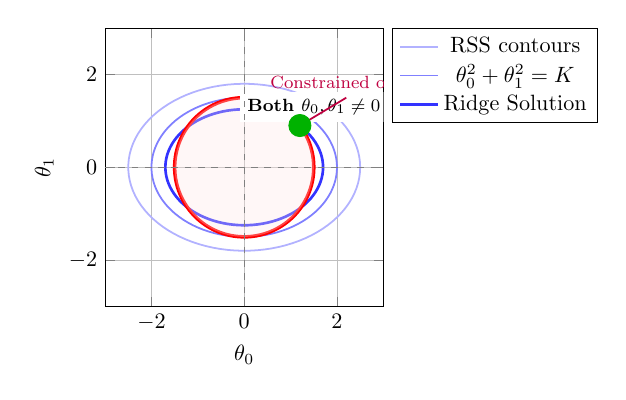
\begin{tikzpicture}[scale=0.8]
\begin{axis}[
    width=6cm, height=6cm,
    xlabel={$\theta_0$}, ylabel={$\theta_1$},
    xmin=-3, xmax=3, ymin=-3, ymax=3,
    axis equal,
    grid=major,
    legend pos=outer north east
]
% Multiple RSS ellipses for better visualization
\addplot[domain=0:360, samples=100, thick, blue!30] ({2.5*cos(x)}, {1.8*sin(x)});
\addplot[domain=0:360, samples=100, thick, blue!50] ({2.0*cos(x)}, {1.5*sin(x)});
\addplot[domain=0:360, samples=100, very thick, blue!80] ({1.7*cos(x)}, {1.25*sin(x)});
\addlegendentry{RSS contours}

% L2 constraint circle with emphasis
\addplot[domain=0:360, samples=100, ultra thick, red] ({1.5*cos(x)}, {1.5*sin(x)});
\addlegendentry{$\theta_0^2 + \theta_1^2 = K$}

% Show the constraint region
\fill[red!10, opacity=0.3] (0,0) circle [radius=1.5];

% Intersection point (not on axis) with annotation
\addplot[only marks, mark=*, mark size=5pt, color=green!70!black] coordinates {(1.2, 0.9)};
\addlegendentry{Ridge Solution}
\node[fill=white] at (axis cs:1.5,1.3) {\footnotesize \textbf{Both $\theta_0, \theta_1 \neq 0$}};

% Add arrows showing the optimization direction
\draw[->, thick, purple] (2.2,1.5) -- (1.2,0.9);
\node at (axis cs:2.5,1.8) {\footnotesize \color{purple} Constrained optimum};

% Mark the axes
\draw[dashed, gray] (-3,0) -- (3,0);
\draw[dashed, gray] (0,-3) -- (0,3);
\end{axis}
\end{tikzpicture}
\end{figure}
\end{column}
\begin{column}{0.4\textwidth}
\begin{keypointsbox}{L2 Constraint Properties}
\begin{itemize}
\item \textbf{Shape:} Perfect circle
\item \textbf{Boundary:} Smooth everywhere
\item \textbf{Intersection:} Rarely on axes
\item \textbf{Result:} No sparsity
\item \textbf{Effect:} Shrinks coefficients proportionally
\end{itemize}
\end{keypointsbox}
\end{column}
\end{columns}
\end{frame}

\begin{frame}{L1 Norm: Lasso Regression}
\begin{columns}
\begin{column}{0.6\textwidth}
\begin{figure}
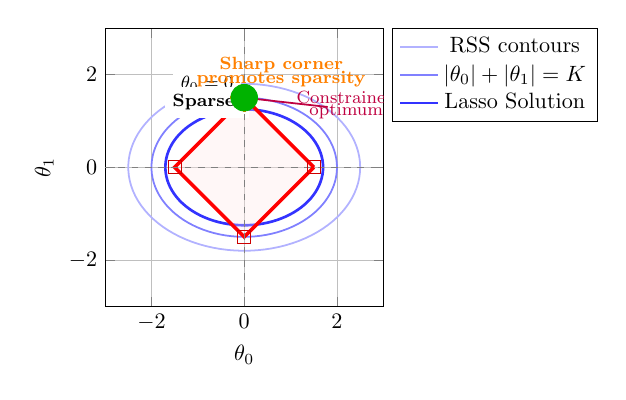
\begin{tikzpicture}[scale=0.8]
\begin{axis}[
    width=6cm, height=6cm,
    xlabel={$\theta_0$}, ylabel={$\theta_1$},
    xmin=-3, xmax=3, ymin=-3, ymax=3,
    axis equal,
    grid=major,
    legend pos=outer north east
]
% Multiple RSS ellipses for consistency
\addplot[domain=0:360, samples=100, thick, blue!30] ({2.5*cos(x)}, {1.8*sin(x)});
\addplot[domain=0:360, samples=100, thick, blue!50] ({2.0*cos(x)}, {1.5*sin(x)});
\addplot[domain=0:360, samples=100, very thick, blue!80] ({1.7*cos(x)}, {1.25*sin(x)});
\addlegendentry{RSS contours}

% Enhanced L1 constraint diamond
\addplot[ultra thick, red, fill=red!10, fill opacity=0.3] coordinates {(1.5,0) (0,1.5) (-1.5,0) (0,-1.5) (1.5,0)};
\addlegendentry{$|\theta_0| + |\theta_1| = K$}

% Highlight the sharp corners
\addplot[only marks, mark=square, mark size=3pt, color=red!80!black] coordinates {(1.5,0) (0,1.5) (-1.5,0) (0,-1.5)};

% Intersection point (on axis) with emphasis
\addplot[only marks, mark=*, mark size=6pt, color=green!70!black] coordinates {(0, 1.5)};
\addlegendentry{Lasso Solution}
\node[fill=white] at (axis cs:-0.8,1.8) {\footnotesize \textbf{$\theta_0 = 0$}};
\node[fill=white] at (axis cs:-0.8,1.4) {\footnotesize \textbf{Sparse!}};

% Add arrow showing optimization direction
\draw[->, thick, purple] (1.8,1.3) -- (0,1.5);
\node at (axis cs:2.2,1.5) {\footnotesize \color{purple} Constrained};
\node at (axis cs:2.2,1.2) {\footnotesize \color{purple} optimum};

% Emphasize the corner where intersection occurs
\draw[very thick, orange, dashed] (-0.3,1.5) -- (0.3,1.5);
\draw[very thick, orange, dashed] (0,1.2) -- (0,1.8);
\node at (axis cs:0.8,2.2) {\footnotesize \color{orange} \textbf{Sharp corner}};
\node at (axis cs:0.8,1.9) {\footnotesize \color{orange} \textbf{promotes sparsity}};

% Mark the axes
\draw[dashed, gray] (-3,0) -- (3,0);
\draw[dashed, gray] (0,-3) -- (0,3);
\end{axis}
\end{tikzpicture}
\end{figure}
\end{column}
\begin{column}{0.4\textwidth}
\begin{keypointsbox}{L1 Constraint Properties}
\begin{itemize}
\item \textbf{Shape:} Diamond/rhombus
\item \textbf{Corners:} Sharp at axes
\item \textbf{Intersection:} High probability on axes
\item \textbf{Result:} Automatic sparsity!
\item \textbf{Effect:} Sets coefficients to exactly zero
\end{itemize}
\end{keypointsbox}
\end{column}
\end{columns}
\end{frame}

\begin{frame}{$L_p$ Norm: $0 < p < 1$ (Example: $p=0.5$)}
\begin{columns}
\begin{column}{0.6\textwidth}
\begin{figure}
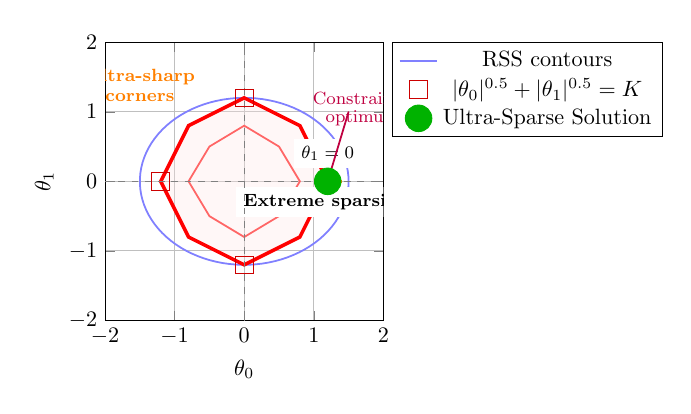
\begin{tikzpicture}[scale=0.8]
\begin{axis}[
    width=6cm, height=6cm,
    xlabel={$\theta_0$}, ylabel={$\theta_1$},
    xmin=-2, xmax=2, ymin=-2, ymax=2,
    axis equal,
    grid=major,
    legend pos=outer north east
]
% RSS ellipse for consistency
\addplot[domain=0:360, samples=100, thick, blue!50] ({1.5*cos(x)}, {1.2*sin(x)});
\addlegendentry{RSS contours}

% Enhanced L_p constraint visualization (p=0.5)
% Create a more accurate representation of the L_0.5 "ball"
\draw[ultra thick, red, fill=red!10, fill opacity=0.3] 
    (1.2,0) -- (0.8,0.8) -- (0,1.2) -- (-0.8,0.8) -- (-1.2,0) -- 
    (-0.8,-0.8) -- (0,-1.2) -- (0.8,-0.8) -- cycle;
\addlegendentry{$|\theta_0|^{0.5} + |\theta_1|^{0.5} = K$}

% Show multiple levels for better understanding
\draw[thick, red!60] (0.8,0) -- (0.5,0.5) -- (0,0.8) -- (-0.5,0.5) -- (-0.8,0) -- (-0.5,-0.5) -- (0,-0.8) -- (0.5,-0.5) -- cycle;

% Emphasize the extremely sharp corners
\addplot[only marks, mark=square, mark size=4pt, color=red!80!black] coordinates {(1.2,0) (0,1.2) (-1.2,0) (0,-1.2)};

% Intersection point (on axis) with strong emphasis
\addplot[only marks, mark=*, mark size=6pt, color=green!70!black] coordinates {(1.2, 0)};
\addlegendentry{Ultra-Sparse Solution}
\node[fill=white] at (axis cs:1.2,0.4) {\footnotesize \textbf{$\theta_1 = 0$}};
\node[fill=white] at (axis cs:1.2,-0.3) {\footnotesize \textbf{Extreme sparsity!}};

% Add arrows and annotations
\draw[->, thick, purple] (1.5,1.0) -- (1.2,0);
\node at (axis cs:1.7,1.2) {\footnotesize \color{purple} Constrained};
\node at (axis cs:1.7,0.9) {\footnotesize \color{purple} optimum};

% Highlight the ultra-sharp corner
\node at (axis cs:-1.5,1.5) {\footnotesize \color{orange} \textbf{Ultra-sharp}};
\node at (axis cs:-1.5,1.2) {\footnotesize \color{orange} \textbf{corners}};
\draw[orange, very thick] (1.1,-0.1) -- (1.1,0.1);
\draw[orange, very thick] (1.0,0) -- (1.4,0);

% Mark the axes
\draw[dashed, gray] (-2,0) -- (2,0);
\draw[dashed, gray] (0,-2) -- (0,2);
\end{axis}
\end{tikzpicture}
\end{figure}
\end{column}
\begin{column}{0.4\textwidth}
\begin{keypointsbox}{$L_p$ Properties $(p<1)$}
\begin{itemize}
\item \textbf{Shape:} Highly concave
\item \textbf{Corners:} Ultra-sharp at axes
\item \textbf{Sparsity:} Extremely high probability
\item \textbf{Optimization:} Non-convex, much harder
\item \textbf{Trade-off:} Better sparsity but computational difficulty
\end{itemize}
\end{keypointsbox}
\end{column}
\end{columns}
\end{frame}

\begin{frame}{Sparsity Trend: $L_2 \to L_1 \to L_p$}
\begin{theorembox}{Key Insight}
As $p$ decreases from 2 to 1 to $p < 1$:
\begin{itemize}
\item Constraint regions become more \textbf{pointed} at axes
\item Probability of intersection at axes \textbf{increases}
\item Sparsity \textbf{increases}
\item Optimization difficulty \textbf{increases}
\end{itemize}
\end{theorembox}
\pause

\begin{alertbox}{Why $p = 1$ is Special}
\begin{itemize}
\item Still promotes sparsity (sharp corners)
\item Remains convex (unlike $p < 1$)
\item Computationally tractable
\end{itemize}
\end{alertbox}
\end{frame}

\subsection{Gradient Descent Interpretation}

\begin{frame}{L2 vs L1: Gradient Descent Behavior}
\begin{columns}
\begin{column}{0.5\textwidth}
\begin{keypointsbox}{L2 Penalty: $f(\theta) = \frac{1}{2}\theta^2$}
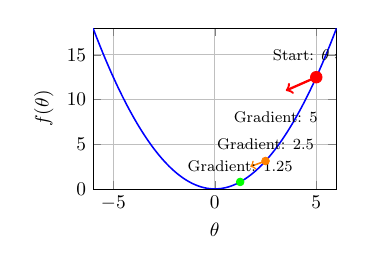
\begin{tikzpicture}[scale=0.7]
\begin{axis}[
    width=6cm, height=4.5cm,
    xlabel={$\theta$}, ylabel={$f(\theta)$},
    xmin=-6, xmax=6, ymin=0, ymax=18,
    grid=major
]
% L2 function
\addplot[domain=-6:6, samples=100, thick, blue] {0.5*x^2};

% Show gradient arrows
\addplot[only marks, mark=*, mark size=3pt, color=red] coordinates {(5, 12.5)};
\draw[red, very thick, ->] (axis cs:5,12.5) -- (axis cs:3.5,11);
\node at (axis cs:5,15) {\footnotesize Start: $\theta=5$};
\node at (axis cs:3,8) {\footnotesize Gradient: $5$};

% Show decreasing gradient
\addplot[only marks, mark=*, mark size=2pt, color=orange] coordinates {(2.5, 3.125)};
\draw[orange, thick, ->] (axis cs:2.5,3.125) -- (axis cs:1.75,2.5);
\node at (axis cs:2.5,5) {\footnotesize Gradient: $2.5$};

\addplot[only marks, mark=*, mark size=2pt, color=green] coordinates {(1.25, 0.78)};
\node at (axis cs:1.25,2.5) {\footnotesize Gradient: $1.25$};
\end{axis}
\end{tikzpicture}
\end{keypointsbox}
\end{column}

\begin{column}{0.5\textwidth}
\begin{keypointsbox}{L1 Penalty: $f(\theta) = |\theta|$}
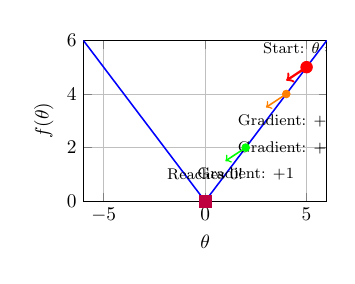
\begin{tikzpicture}[scale=0.7]
\begin{axis}[
    width=6cm, height=4.5cm,
    xlabel={$\theta$}, ylabel={$f(\theta)$},
    xmin=-6, xmax=6, ymin=0, ymax=6,
    grid=major
]
% L1 function
\addplot[domain=-6:0, samples=100, thick, blue] {-x};
\addplot[domain=0:6, samples=100, thick, blue] {x};

% Show constant gradient arrows
\addplot[only marks, mark=*, mark size=3pt, color=red] coordinates {(5, 5)};
\draw[red, very thick, ->] (axis cs:5,5) -- (axis cs:4,4.5);
\node at (axis cs:5,5.7) {\footnotesize Start: $\theta=5$};
\node at (axis cs:4,3) {\footnotesize Gradient: $+1$};

\addplot[only marks, mark=*, mark size=2pt, color=orange] coordinates {(4, 4)};
\draw[orange, thick, ->] (axis cs:4,4) -- (axis cs:3,3.5);
\node at (axis cs:4,2) {\footnotesize Gradient: $+1$};

\addplot[only marks, mark=*, mark size=2pt, color=green] coordinates {(2, 2)};
\draw[green, thick, ->] (axis cs:2,2) -- (axis cs:1,1.5);
\node at (axis cs:2,1) {\footnotesize Gradient: $+1$};

% Mark the corner
\addplot[only marks, mark=square*, mark size=3pt, color=purple] coordinates {(0, 0)};
\node at (axis cs:0,1) {\footnotesize Reaches 0!};
\end{axis}
\end{tikzpicture}
\end{keypointsbox}
\end{column}
\end{columns}

\begin{examplebox}{Key Difference}
L2: Gradient $\propto \theta$ (decreases). L1: Constant gradient $= \pm 1$
\end{examplebox}
\end{frame}

\begin{frame}{Gradient Descent: Step 1}
\begin{columns}
\begin{column}{0.5\textwidth}
\begin{codebox}{L2 Update}
\begin{itemize}
\item $\frac{df}{d\theta} = \theta = 5$
\item $\theta_{new} = 5 - 0.5 \times 5 = 2.5$
\item $f(2.5) = 3.125$
\end{itemize}
\end{codebox}
\end{column}

\begin{column}{0.5\textwidth}
\begin{codebox}{L1 Update}
\begin{itemize}
\item $\frac{df}{d\theta} = \text{sign}(\theta) = +1$
\item $\theta_{new} = 5 - 0.5 \times 1 = 4.5$
\item $f(4.5) = 4.5$
\end{itemize}
\end{codebox}
\end{column}
\end{columns}

\begin{alertbox}{Key Difference}
L2 gradient depends on $\theta$ value, L1 gradient is constant $\pm 1$
\end{alertbox}
\end{frame}

\begin{frame}{Gradient Descent: Multiple Steps}
\begin{columns}
\begin{column}{0.5\textwidth}
\begin{keypointsbox}{L2 Sequence}
\begin{itemize}
\item $\theta_0 = 5.0$
\item $\theta_1 = 2.5$ 
\item $\theta_2 = 1.25$
\item $\theta_3 = 0.625$
\item $\theta_4 = 0.3125$
\item $\vdots$ (never exactly 0)
\end{itemize}
\end{keypointsbox}
\end{column}

\begin{column}{0.5\textwidth}
\begin{keypointsbox}{L1 Sequence}
\begin{itemize}
\item $\theta_0 = 5.0$
\item $\theta_1 = 4.5$
\item $\theta_2 = 4.0$
\item $\theta_3 = 3.5$
\item $\vdots$
\item $\theta_{10} = 0.0$ (exactly!)
\end{itemize}
\end{keypointsbox}
\end{column}
\end{columns}

\begin{theorembox}{Sparsity Mechanism}
L1 penalty creates \textbf{constant gradient} that drives parameters to exactly zero in finite steps!
\end{theorembox}
\end{frame}

\section{Geometric Interpretation}

\begin{frame}{Sample Dataset for Demonstration}
\begin{examplebox}{True Function}
We'll demonstrate Lasso on a simple linear relationship: $y = 4x + 7$
\end{examplebox}

\begin{figure}
    \centering
    \includegraphics[width=0.65\linewidth]{../assets/lasso-regression/figures/true_function.pdf}
    \caption{{\footnotesize Sample data from $y = 4x + 7$ with noise}}
    \label{fig:my_label}
\end{figure}
\end{frame}

\begin{frame}{Geometric Interpretation: L1 vs L2 Constraints}
\begin{figure}
    \centering
    \includegraphics[width=0.6\linewidth]{../assets/lasso-regression/figures/lasso_base_contour.pdf}
    \caption{{\footnotesize L1 vs L2 constraint regions}}
    \label{fig:my_label}
\end{figure}

\begin{keypointsbox}{Key Insight}
{\footnotesize
Diamond corners $\Rightarrow$ exact zeros! Circle $\Rightarrow$ no sparsity.
}
\end{keypointsbox}
\end{frame}

\section{Regularization Effects}

\begin{frame}{Effect of $\lambda$ on Solution Path}
\begin{alertbox}{Regularization Parameter}
$\lambda$ controls fit vs sparsity trade-off
\end{alertbox}

\begin{figure}
\includegraphics[width=0.75\linewidth]{../assets/lasso-regression/figures/lasso_1.0.pdf}
\caption{{\footnotesize $\lambda = 1.0$ - Moderate regularization}}
\end{figure}
\end{frame}

\begin{frame}{Increasing Regularization: $\lambda = 1.25$}
\begin{figure}\includegraphics[width=0.75\linewidth]{../assets/lasso-regression/figures/lasso_1.25.pdf}\caption{{\footnotesize $\lambda = 1.25$ - Higher regularization}}
\end{figure}

\begin{keypointsbox}{Observation}
As $\lambda$ increases $\rightarrow$ solution becomes sparser
\end{keypointsbox}
\end{frame}

\begin{frame}{Further Regularization: $\lambda = 1.5$}
\begin{figure}\includegraphics[width=0.75\linewidth]{../assets/lasso-regression/figures/lasso_1.5.pdf}\caption{{\footnotesize $\lambda = 1.5$ - Even higher regularization}}
\end{figure}

\begin{alertbox}{Sparsity Effect}
More coefficients $\rightarrow$ exactly zero
\end{alertbox}
\end{frame}

\begin{frame}{High Regularization: $\lambda = 1.75$}
\begin{figure}\includegraphics[width=0.75\linewidth]{../assets/lasso-regression/figures/lasso_1.75.pdf}\caption{{\footnotesize $\lambda = 1.75$ - Strong regularization}}
\end{figure}

\begin{codebox}{Feature Selection}
Automatic selection of most important features
\end{codebox}
\end{frame}


\begin{frame}{Maximum Regularization: $\lambda = 2.0$}
\begin{figure}\includegraphics[width=0.75\linewidth]{../assets/lasso-regression/figures/lasso_2.0.pdf}\caption{{\footnotesize $\lambda = 2.0$ - Very strong regularization}}
\end{figure}

\begin{alertbox}{Extreme Sparsity}
Only most crucial features remain non-zero
\end{alertbox}
\end{frame}



%\begin{frame}{Why Lasso Gives Sparse solution}
%\begin{figure}
%    \centering
%    \includegraphics[scale = 0.4]{Lasso/lasso_2.png}
%    \label{fig:my_label}
%\end{figure}
%\begin{itemize}
%\small{
%    \item Pointedness of $L_{p}$ norm 
%    \item  Probability of Intersecting an axis increases.
%    \item Sparsity increases. 
%    \item Solving difficulty also increases
%    }
%\end{itemize}
%
%\end{frame}
%
%\begin{frame}{Interpretation : II}
%\begin{figure}
%    \centering
%    \includegraphics[scale = 0.3]{Lasso/lasso_3.png}
%    \label{fig:my_label}
%\end{figure}
%
%\end{frame}
%
%
%
%\begin{frame}{Gradient Descent}
%
%
%\foreach \x in {0,1,2,3,4} 
%{%
%\includegraphics<\x>[scale=0.75]{Lasso/GD_iteration_\x.pdf}
%%    
%}
%
%
%\end{frame}

\begin{frame}{Lasso Regularization Path}
\begin{figure}
    \centering
    \includegraphics[width=0.7\linewidth]{../assets/lasso-regression/figures/lasso_reg.pdf}
    \caption{{\footnotesize Coefficient values vs $\lambda$}}
    \label{fig:my_label}
\end{figure}

\begin{keypointsbox}{Key Observations}
{\small
\begin{itemize}
\item Coefficients shrink to zero as $\lambda$ increases
\item Different coefficients zero at different $\lambda$
\item Natural feature selection ordering
\end{itemize}
}
\end{keypointsbox}
\end{frame}


\section{Feature Selection Properties}

\begin{frame}{Lasso for Automatic Feature Selection}
\begin{definitionbox}{Automatic Feature Selection}
Lasso performs regression and feature selection simultaneously by setting irrelevant coefficients to exactly zero
\end{definitionbox}

\begin{keypointsbox}{Key Advantages}
{\small
\begin{itemize}
\item \textbf{Sparsity}: Many coefficients $\rightarrow$ exactly zero
\item \textbf{Interpretability}: Understand which features matter
\item \textbf{Efficiency}: Fewer parameters, faster prediction
\end{itemize}
}
\end{keypointsbox}
\end{frame}

\begin{frame}{Real-World Feature Selection}
\begin{examplebox}{Genomics Example}
Start with 20,000 genes $\rightarrow$ Lasso selects 50 relevant ones
\end{examplebox}

\begin{keypointsbox}{Other Applications}
{\small
\begin{itemize}
\item Text mining: 100k+ words $\rightarrow$ select key terms
\item Finance: 1000+ indicators $\rightarrow$ find predictive signals
\item Image processing: millions of pixels $\rightarrow$ identify features
\end{itemize}
}
\end{keypointsbox}
\end{frame}

\section{Subgradient Methods}

\begin{frame}{What is a Subgradient?}
\begin{definitionbox}{Subgradient}
A subgradient generalizes the concept of gradient to convex but non-differentiable functions
\end{definitionbox}
\pause

\begin{examplebox}{Classic Example}
For $f(x) = |x|$:
\begin{itemize}
\item $f'(x) = 1$ when $x > 0$
\item $f'(x) = -1$ when $x < 0$  
\item $f'(0)$ is undefined, but subgradient $\in [-1, 1]$
\end{itemize}
\end{examplebox}
\pause

\begin{alertbox}{Why Important for Lasso?}
The L1 penalty $|\theta_j|$ is non-differentiable at $\theta_j = 0$
\end{alertbox}
\end{frame}

\begin{frame}{Subgradient: Visual Intuition}
\begin{alertbox}{Task}
Find the "derivative" of $f(x)$ at the non-differentiable point $x = x_0$
\end{alertbox}

\begin{figure}
\centering
\includegraphics[width=0.6\linewidth]{../assets/lasso-regression/diagrams/subgradient_1.jpg}
\caption{{\footnotesize Non-differentiable function at $x_0$}}
\label{fig:Non-differentiable function}
\end{figure}
\end{frame}

\begin{frame}{Subgradient Construction}
\begin{codebox}{Construction Method}
Find a differentiable function $g(x)$ such that:
\begin{itemize}
\item $g(x_0) = f(x_0)$ (intersects at the point)
\item $g(x) \leq f(x)$ for all $x$ (lies below or on $f$)
\end{itemize}
\end{codebox}

\begin{figure}
\centering
\includegraphics[width=0.55\linewidth]{../assets/lasso-regression/diagrams/subgradient_2.jpg}
\caption{{\footnotesize Supporting hyperplane construction}}
\label{fig:my_label}
\end{figure}
\end{frame}

\begin{frame}{Computing the Subgradient}
\begin{theorembox}{Subgradient Definition}
Slope of $g(x)$ at $x = x_0$ gives subgradient of $f$ at $x_0$
\end{theorembox}

\begin{figure}
\centering
\includegraphics[width=0.5\linewidth]{../assets/lasso-regression/diagrams/subgradient_2.jpg}
\caption{{\footnotesize Slope $\rightarrow$ subgradient}}
\label{fig:my_label}
\end{figure}
\end{frame}

\begin{frame}{Subgradient Sets}
\begin{keypointsbox}{Key Insight}
Multiple supporting lines $\Rightarrow$ set of valid subgradients
\end{keypointsbox}

\begin{examplebox}{For $f(x) = |x|$}
At $x = 0$: subgradient set is $[-1, +1]$
\end{examplebox}
\end{frame}

\begin{frame}{Example: Subgradient of $f(x) = |x|$}
\begin{codebox}{Subgradient Set}
For $f(x) = |x|$ at $x = 0$:
$$\partial f(0) = [-1, 1]$$
\end{codebox}

\begin{figure}
\centering
\includegraphics[width=0.5\linewidth]{../assets/lasso-regression/diagrams/subgradient_3.jpg}
\caption{{\footnotesize Lines with slope in $[-1,1]$ support $|x|$ at $x=0$}}
\label{fig:my_label}
\end{figure}
\end{frame}

\begin{frame}{Connection to Lasso}
\begin{alertbox}{Lasso Connection}
This subgradient concept is exactly what we need for the L1 penalty term!
\end{alertbox}

\begin{keypointsbox}{Next Step}
We'll use subgradients to derive coordinate descent for Lasso
\end{keypointsbox}
\end{frame}

\section{Coordinate Descent Algorithm}

\begin{frame}{Introduction to Coordinate Descent}
\begin{definitionbox}{Coordinate Descent}
Optimization method: minimize one coordinate at a time
\end{definitionbox}
\pause

\begin{keypointsbox}{Key Idea}
{\footnotesize
\begin{itemize}
\item Hard: optimize all coordinates together
\item Easy: optimize one coordinate at a time
\item Perfect for non-differentiable Lasso!
\end{itemize}
}
\end{keypointsbox}
\end{frame}

\begin{frame}{Coordinate Descent Algorithm}
\begin{codebox}{Algorithm Overview}
$$\min_{\vtheta} f(\vtheta) \text{ becomes } \min_{\theta_j} f(\theta_1, \ldots, \theta_{j-1}, \theta_j, \theta_{j+1}, \ldots, \theta_d)$$
\end{codebox}

\begin{alertbox}{Process}
Cycle through coordinates, optimizing one at a time
\end{alertbox}
\end{frame}

%{
%\setbeamercolor{background canvas}{bg=}
%\includepdf[page=-]{coordinate-vis.pdf}
%}


\begin{frame}{Coordinate Descent Properties}
\begin{keypointsbox}{Advantages}
{\footnotesize
\begin{itemize}
\item \textbf{No step-size}: Exact 1D minimization
\item \textbf{Convergence}: Guaranteed for convex Lasso
\item \textbf{Efficient}: Closed-form updates
\end{itemize}
}
\end{keypointsbox}
\pause

\begin{codebox}{Selection Strategies}
{\footnotesize Cyclic, Random, or Greedy coordinate selection}
\end{codebox}
\end{frame}




\section{Worked Example}

\begin{frame}{Coordinate Descent Example Setup}
\begin{examplebox}{Problem}
Learn $y = \theta_0 + \theta_1 x$ using coordinate descent on the dataset below
\end{examplebox}

\begin{table}[]
\centering
\label{tab:my-table}
\begin{tabular}{|c|c|}
\hline
\textbf{x} & \textbf{y} \\ \hline
1 & 1 \\ \hline
2 & 2 \\ \hline
3 & 3 \\ \hline
\end{tabular}
\end{table}

\begin{codebox}{Initial Conditions}
\begin{itemize}
\item Initial parameters: $(\theta_0, \theta_1) = (2,3)$
\item We'll run for 2 iterations
\item Using standard least squares (no regularization for simplicity)
\end{itemize}
\end{codebox}
\end{frame}



\begin{frame}{Coordinate Descent : Example}
Our predictor, $\hat{y} = \theta_0 + \theta_1x$\\
\vspace{1cm}
Error for $i^{th}$ datapoint, $\epsilon_i = y_i - \hat{y_i}$\\
$\epsilon_1 = 1 - \theta_0 - \theta_1$ \\
$\epsilon_2 = 2 - \theta_0 - 2\theta_1$ \\
$\epsilon_3 = 3 - \theta_0 - 3\theta_1$ \\

\vspace{1cm}
$\MSE = \frac{\epsilon_1^2 + \epsilon_2^2 + \epsilon_3^2}{3} = \frac{14 + 3\theta_0^2 + 14\theta_1^2 -12\theta_0 - 28\theta_1 + 12\theta_0\theta_1}{3}$\\
\end{frame}





\begin{frame}{Iteration 0}

MSE = $\frac{1}{3}(14+3\theta_{0}^{2}+14\theta_{1}^{2}-12\theta_{0}-28\theta_{1}+12\theta_{0}\theta_{1})$\\

\begin{columns}
\begin{column}{0.6\textwidth}
\begin{adjustbox}{max totalsize={\textwidth},center}
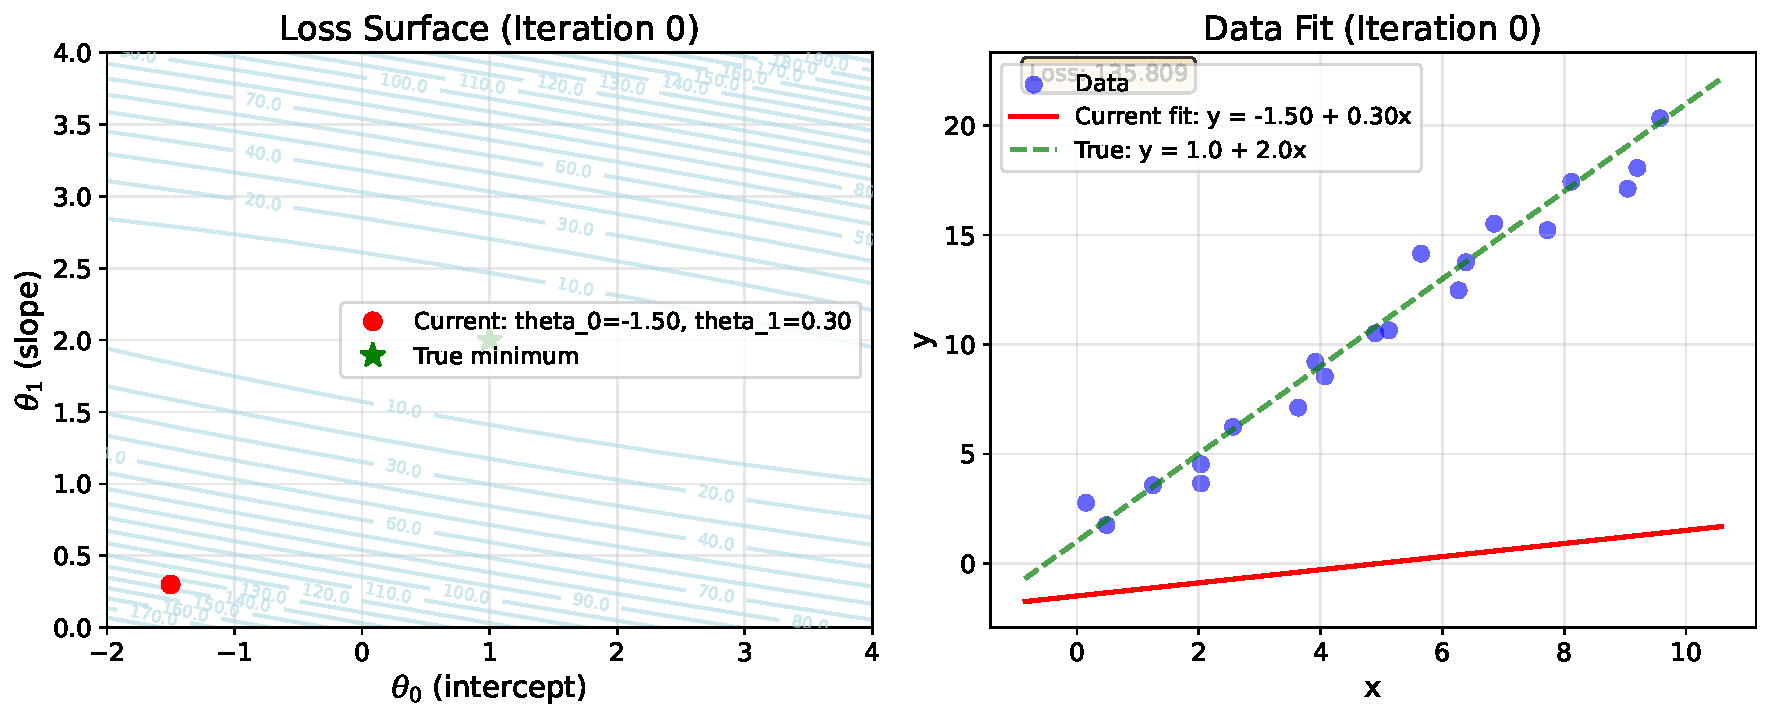
\includegraphics[width=\textwidth]{../../maths/assets/mathematical-ml/figures/gradient-descent-0.pdf}
\end{adjustbox}

\end{column}
\begin{column}{0.5\textwidth}
\begin{adjustbox}{max totalsize={\textwidth},center}
\includegraphics[width=\textwidth]{../../maths/assets/mathematical-ml/figures/contour-linreg-0.pdf}
\end{adjustbox}
\end{column}
\end{columns}




\end{frame}

\begin{frame}{Coordinate Descent : Example}
\textbf{Iteration 1}\\
\vspace{0.5cm}
INIT: $\theta_{0} = 2$ and  $\theta_{1}  = 3$\\

\vspace{0.5cm}
$\theta_1 = 3$ optimize for $\theta_{0}$\\ 
\only<2->{
\vspace{0.5cm}
$\frac{\partial \MSE}{\partial \theta_{0}} = 6\theta_0 + 24 = 0$\\
\vspace{0.5cm}
$\theta_0 = -4$


}


\end{frame}


\begin{frame}{Iteration 1}

MSE = $\frac{1}{3}(14+3\theta_{0}^{2}+14\theta_{1}^{2}-12\theta_{0}-28\theta_{1}+12\theta_{0}\theta_{1})$\\

\begin{columns}
\begin{column}{0.6\textwidth}
\begin{adjustbox}{max totalsize={\textwidth},center}
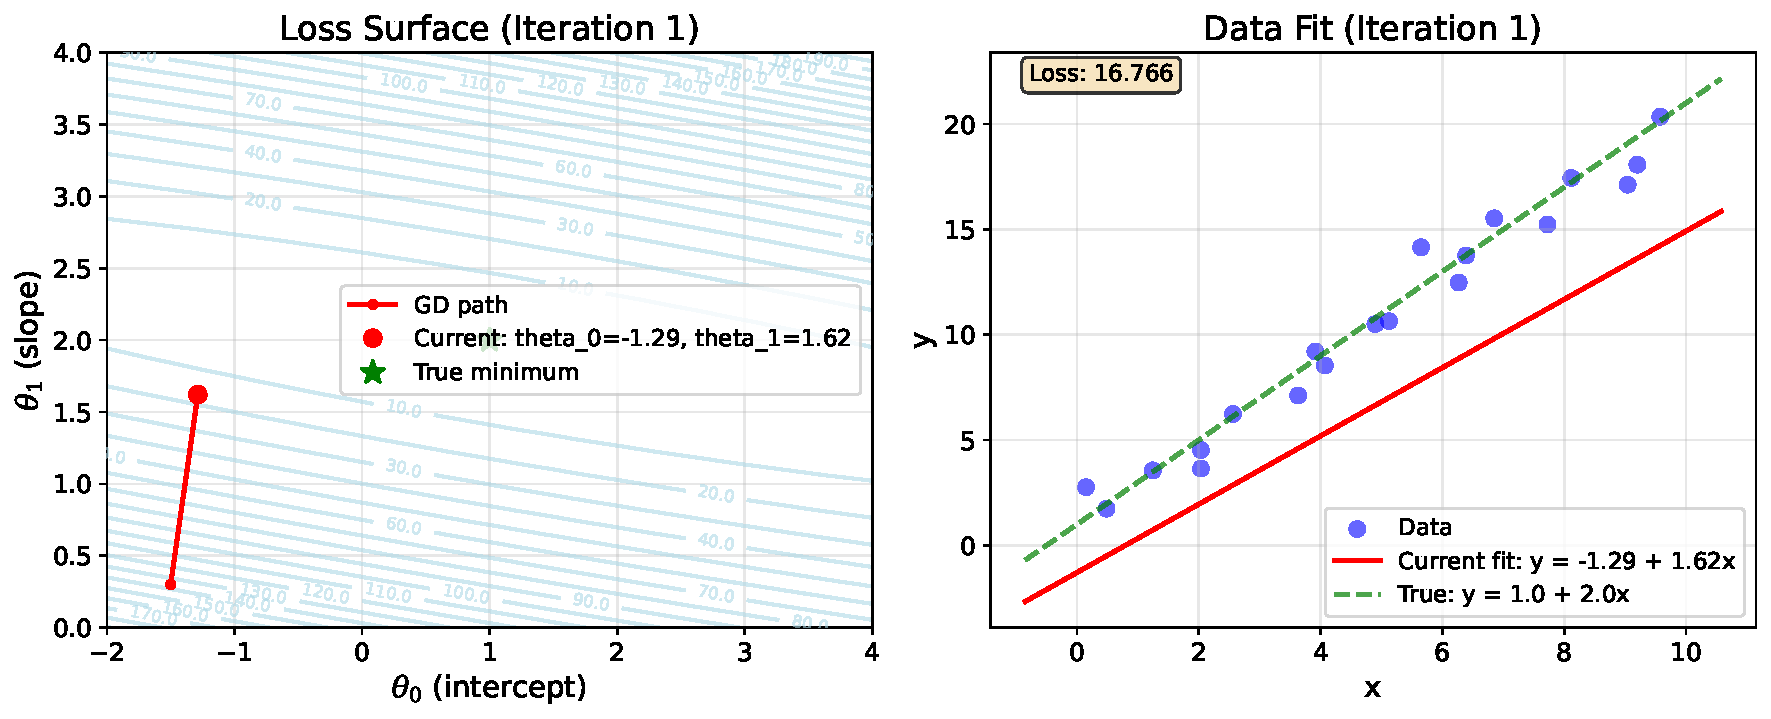
\includegraphics[width=\textwidth]{../../maths/assets/mathematical-ml/figures/gradient-descent-1.pdf}
\end{adjustbox}

\end{column}
\begin{column}{0.5\textwidth}
\begin{adjustbox}{max totalsize={\textwidth},center}
\includegraphics[width=\textwidth]{../../maths/assets/mathematical-ml/figures/contour-linreg-1.pdf}
\end{adjustbox}
\end{column}
\end{columns}


\end{frame}

\begin{frame}{Coordinate Descent : Example}
\textbf{Iteration 2}\\
\vspace{0.5cm}
INIT: $\theta_{0} = -4$ and  $\theta_{1}  = 3$\\

\vspace{0.5cm}
$\theta_0 = -4$ optimize for $\theta_{1}$\\ 
\only<2->{
\vspace{0.5cm}
$\theta_1 = 2.7$
}


\end{frame}


\begin{frame}{Iteration 2}

MSE = $\frac{1}{3}(14+3\theta_{0}^{2}+14\theta_{1}^{2}-12\theta_{0}-28\theta_{1}+12\theta_{0}\theta_{1})$\\

\begin{columns}
\begin{column}{0.6\textwidth}
\begin{adjustbox}{max totalsize={\textwidth},center}
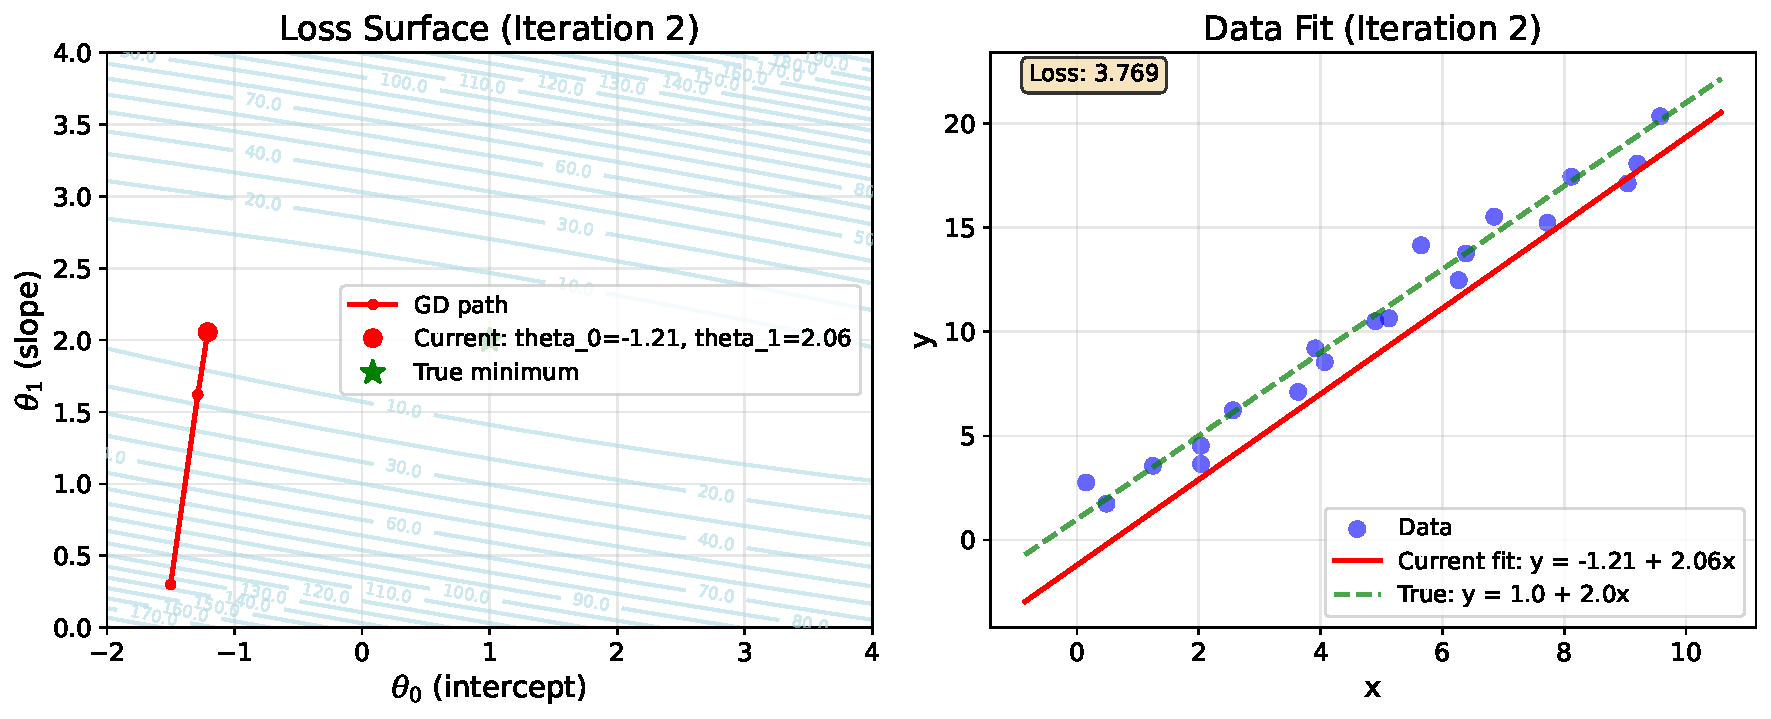
\includegraphics[width=\textwidth]{../../maths/assets/mathematical-ml/figures/gradient-descent-2.pdf}
\end{adjustbox}

\end{column}
\begin{column}{0.5\textwidth}
\begin{adjustbox}{max totalsize={\textwidth},center}
\includegraphics[width=\textwidth]{../../maths/assets/mathematical-ml/figures/contour-linreg-2.pdf}
\end{adjustbox}
\end{column}
\end{columns}


\end{frame}

\begin{frame}{Coordinate Descent : Example}
\textbf{Iteration 3}\\
\vspace{0.5cm}
INIT: $\theta_{0} = -4$ and $\theta_{1}  = 2.7$\\

\vspace{0.5cm}
$\theta_1 = 2.7$ optimize for $\theta_{0}$\\ 
\only<2->{
\vspace{0.5cm}
$\theta_0 = -3.4$
}


\end{frame}

\begin{frame}{Iteration 3}

MSE = $\frac{1}{3}(14+3\theta_{0}^{2}+14\theta_{1}^{2}-12\theta_{0}-28\theta_{1}+12\theta_{0}\theta_{1})$\\

\begin{columns}
\begin{column}{0.6\textwidth}
\begin{adjustbox}{max totalsize={\textwidth},center}
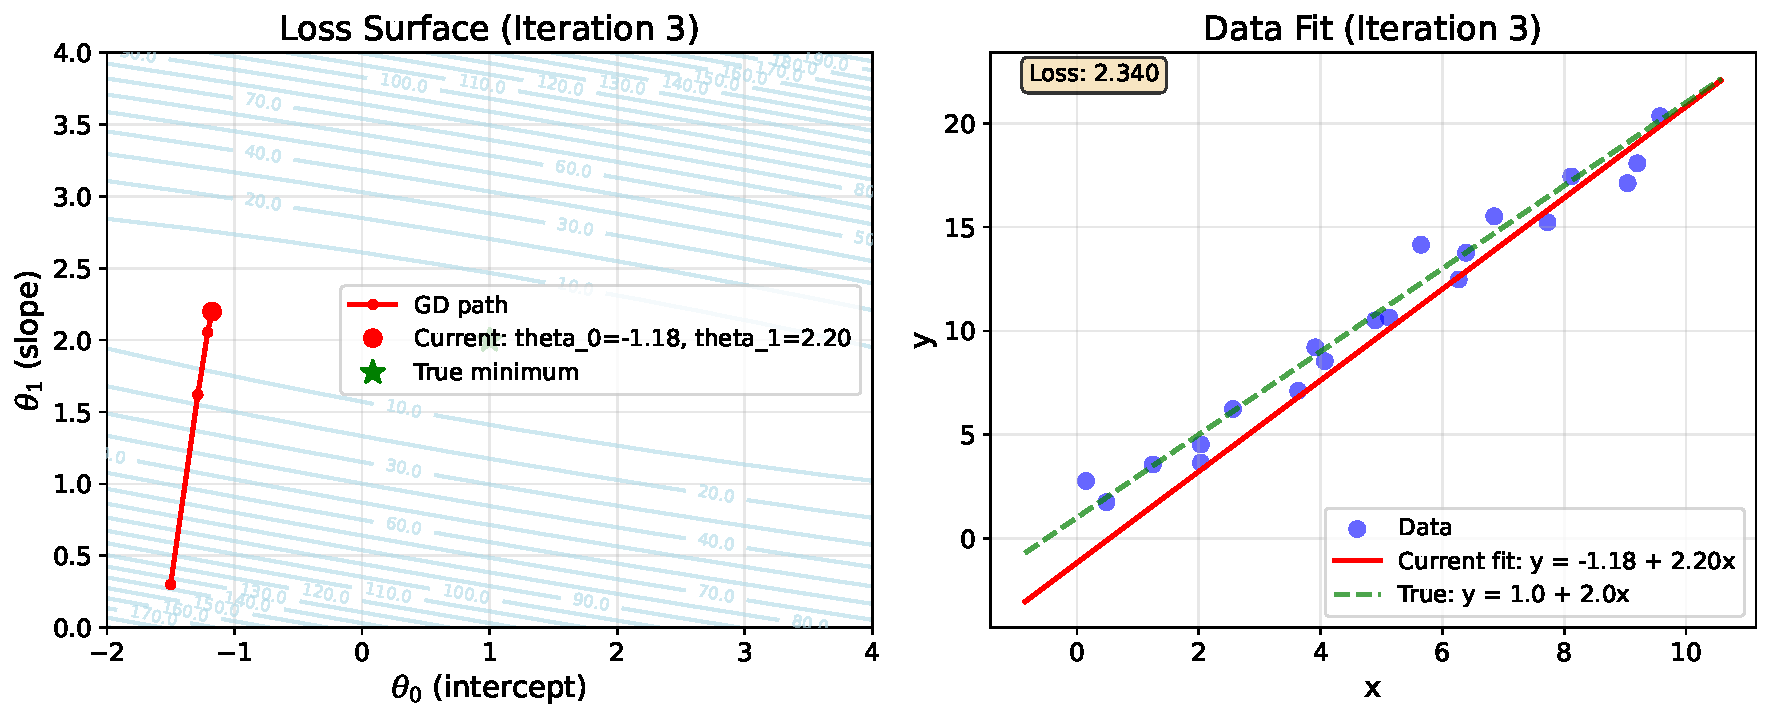
\includegraphics[width=\textwidth]{../../maths/assets/mathematical-ml/figures/gradient-descent-3.pdf}
\end{adjustbox}

\end{column}
\begin{column}{0.5\textwidth}
\begin{adjustbox}{max totalsize={\textwidth},center}
\includegraphics[width=\textwidth]{../../maths/assets/mathematical-ml/figures/contour-linreg-3.pdf}
\end{adjustbox}
\end{column}
\end{columns}


\end{frame}


\section{Visual Coordinate Descent}

\begin{frame}{Coordinate Descent: Visual Algorithm}
\begin{examplebox}{Setup}
Minimize $f(\theta_0, \theta_1) = (\theta_0 - 2)^2 + (\theta_1 - 1)^2$ starting from $(0, 3)$
\end{examplebox}

\begin{figure}
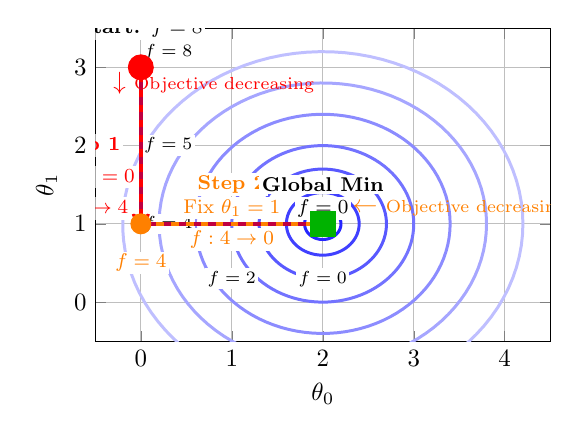
\begin{tikzpicture}[scale=0.9]
\begin{axis}[
    width=8cm, height=6cm,
    xlabel={$\theta_0$}, ylabel={$\theta_1$},
    xmin=-0.5, xmax=4.5, ymin=-0.5, ymax=3.5,
    axis equal=false,
    grid=major,
    colormap/cool
]
% Enhanced contour lines with better visibility and labels
\addplot[domain=0:360, samples=100, very thick, blue!25] ({2 + 2.2*cos(x)}, {1 + 2.2*sin(x)});
\addplot[domain=0:360, samples=100, very thick, blue!35] ({2 + 1.8*cos(x)}, {1 + 1.8*sin(x)});
\addplot[domain=0:360, samples=100, very thick, blue!45] ({2 + 1.4*cos(x)}, {1 + 1.4*sin(x)});
\addplot[domain=0:360, samples=100, very thick, blue!55] ({2 + 1.0*cos(x)}, {1 + 1.0*sin(x)});
\addplot[domain=0:360, samples=100, very thick, blue!65] ({2 + 0.7*cos(x)}, {1 + 0.7*sin(x)});
\addplot[domain=0:360, samples=100, very thick, blue!75] ({2 + 0.4*cos(x)}, {1 + 0.4*sin(x)});
\addplot[domain=0:360, samples=100, very thick, blue!85] ({2 + 0.2*cos(x)}, {1 + 0.2*sin(x)});

% Contour level labels positioned clearly
\node[fill=white, inner sep=1pt] at (axis cs:0.3,3.2) {\scriptsize $f=8$};
\node[fill=white, inner sep=1pt] at (axis cs:0.3,2.0) {\scriptsize $f=5$};
\node[fill=white, inner sep=1pt] at (axis cs:0.3,1.0) {\scriptsize $f=4$};
\node[fill=white, inner sep=1pt] at (axis cs:1.0,0.3) {\scriptsize $f=2$};
\node[fill=white, inner sep=1pt] at (axis cs:2.0,0.3) {\scriptsize $f=0$};

% Starting point with clear marking
\addplot[only marks, mark=*, mark size=5pt, color=red] coordinates {(0, 3)};
\node[fill=white, inner sep=1pt] at (axis cs:0,3.5) {\footnotesize \textbf{Start: $f=8$}};

% Step 1: optimize θ₁ (vertical move showing objective reduction)
\addplot[ultra thick, red, ->] coordinates {(0,3) (0,1)};
\node[fill=white, inner sep=1pt] at (axis cs:-0.6,2) {\footnotesize \color{red} \textbf{Step 1}};
\node[fill=white, inner sep=1pt] at (axis cs:-0.6,1.6) {\footnotesize \color{red} Fix $\theta_0=0$};
\node[fill=white, inner sep=1pt] at (axis cs:-0.6,1.2) {\footnotesize \color{red} $f: 8 \to 4$};

% Intermediate point after step 1 with value
\addplot[only marks, mark=*, mark size=4pt, color=orange] coordinates {(0, 1)};
\node[fill=white, inner sep=1pt] at (axis cs:0,0.5) {\footnotesize \color{orange} $f=4$};

% Step 2: optimize θ₀ (horizontal move showing final reduction)  
\addplot[ultra thick, orange, ->] coordinates {(0,1) (2,1)};
\node[fill=white, inner sep=1pt] at (axis cs:1,1.5) {\footnotesize \color{orange} \textbf{Step 2}};
\node[fill=white, inner sep=1pt] at (axis cs:1,1.2) {\footnotesize \color{orange} Fix $\theta_1=1$};
\node[fill=white, inner sep=1pt] at (axis cs:1,0.8) {\footnotesize \color{orange} $f: 4 \to 0$};

% Global optimum with emphasis
\addplot[only marks, mark=square*, mark size=5pt, color=green!70!black] coordinates {(2, 1)};
\node[fill=white, inner sep=1pt] at (axis cs:2,1.5) {\footnotesize \textbf{Global Min}};
\node[fill=white, inner sep=1pt] at (axis cs:2,1.2) {\footnotesize \textbf{$f=0$}};

% Enhanced path visualization with coordinate-wise movement emphasis
\draw[ultra thick, purple, dashed] (axis cs:0,3) -- (axis cs:0,1) -- (axis cs:2,1);

% Add arrows to show direction of objective reduction
\node at (axis cs:0.8,2.8) {\color{red} $\downarrow$ \scriptsize Objective decreasing};
\node at (axis cs:3.5,1.2) {\color{orange} $\leftarrow$ \scriptsize Objective decreasing};
\end{axis}
\end{tikzpicture}
\end{figure}
\end{frame}

\begin{frame}{Coordinate Descent: Step-by-Step}
\begin{columns}
\begin{column}{0.5\textwidth}
\begin{codebox}{Step 1: Fix $\theta_0 = 0$}
Minimize: $f(0, \theta_1) = 4 + (\theta_1 - 1)^2$
$$\frac{\partial f}{\partial \theta_1} = 2(\theta_1 - 1) = 0$$
$$\theta_1^* = 1$$
\end{codebox}
\end{column}

\begin{column}{0.5\textwidth}
\begin{codebox}{Step 2: Fix $\theta_1 = 1$}  
Minimize: $f(\theta_0, 1) = (\theta_0 - 2)^2$
$$\frac{\partial f}{\partial \theta_0} = 2(\theta_0 - 2) = 0$$
$$\theta_0^* = 2$$
\end{codebox}
\end{column}
\end{columns}

\begin{keypointsbox}{Key Observations}
\begin{itemize}
\item Each step moves parallel to coordinate axes
\item Each step finds exact 1D minimum
\item Converges to global minimum in 2 steps (for this quadratic)
\end{itemize}
\end{keypointsbox}
\end{frame}

\section{When Coordinate Descent Fails}

\begin{frame}{Function: $f(x, y) = |x + y| + 3|y - x|$}
\begin{examplebox}{Problematic Function}
Let's visualize: $f(x, y) = |x + y| + 3|y - x|$ - a non-smooth function with ridges
\end{examplebox}

\begin{figure}
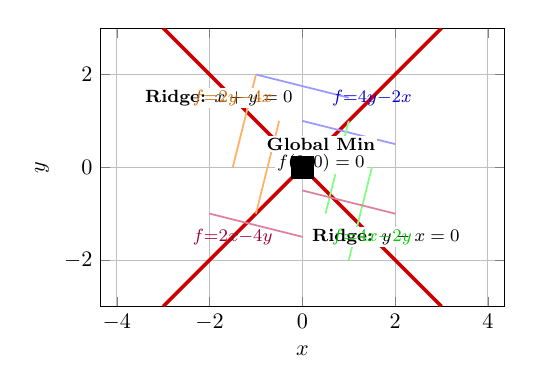
\begin{tikzpicture}[scale=0.8]
\begin{axis}[
    width=8cm, height=6cm,
    xlabel={$x$}, ylabel={$y$},
    xmin=-3, xmax=3, ymin=-3, ymax=3,
    axis equal,
    grid=major,
    view={0}{90}
]
% Create comprehensive contour visualization showing the full function structure
% |x + y| + 3|y - x| has different linear behaviors in 4 regions

% For x+y >= 0 and y-x >= 0: f = (x+y) + 3(y-x) = 4y - 2x
% For x+y >= 0 and y-x <= 0: f = (x+y) + 3(x-y) = 4x - 2y  
% For x+y <= 0 and y-x >= 0: f = -(x+y) + 3(y-x) = 2y - 4x
% For x+y <= 0 and y-x <= 0: f = -(x+y) + 3(x-y) = 2x - 4y

% Draw the ridge lines where the function is non-differentiable
\draw[ultra thick, red!80!black] (-3,-3) -- (3,3);  % x + y = 0 line
\draw[ultra thick, red!80!black] (-3,3) -- (3,-3);   % y - x = 0 line

% Simplified contour representation showing different linear regions
\draw[blue!40, thick] (-1,2) -- (1,1.5);
\draw[blue!40, thick] (0,1) -- (2,0.5);
\draw[green!50, thick] (1,-2) -- (1.5,0);
\draw[green!50, thick] (0.5,-1) -- (1,1);
\draw[orange!60, thick] (-1.5,0) -- (-1,2);
\draw[orange!60, thick] (-1,-1) -- (-0.5,1);
\draw[purple!50, thick] (-2,-1) -- (0,-1.5);
\draw[purple!50, thick] (0,-0.5) -- (2,-1);

% Global minimum with emphasis
\addplot[only marks, mark=square*, mark size=5pt, color=black] coordinates {(0, 0)};
\node[fill=white, inner sep=1pt] at (axis cs:0.4,0.5) {\footnotesize \textbf{Global Min}};
\node[fill=white, inner sep=1pt] at (axis cs:0.4,0.1) {\footnotesize $f(0,0)=0$};

% Label the ridges with better positioning
\node[fill=white, inner sep=1pt] at (axis cs:-1.8,1.5) {\footnotesize \textbf{Ridge:} $x+y=0$};
\node[fill=white, inner sep=1pt] at (axis cs:1.8,-1.5) {\footnotesize \textbf{Ridge:} $y-x=0$};

% Add region labels to show different behaviors with proper formatting
\node at (axis cs:-1.5,1.5) {\footnotesize \color{orange!80!black} $f \mathord{=} 2y\mathord{-}4x$};
\node at (axis cs:1.5,1.5) {\footnotesize \color{blue!80!black} $f \mathord{=} 4y\mathord{-}2x$};
\node at (axis cs:1.5,-1.5) {\footnotesize \color{green!80!black} $f \mathord{=} 4x\mathord{-}2y$};
\node at (axis cs:-1.5,-1.5) {\footnotesize \color{purple!80!black} $f \mathord{=} 2x\mathord{-}4y$};
\end{axis}
\end{tikzpicture}
\end{figure}

\begin{alertbox}{Non-Smooth Surface with Ridges}
Function is piecewise linear with ridges along $x+y=0$ and $y-x=0$. Different gradients in each region!
\end{alertbox}
\end{frame}

\begin{frame}{Coordinate Descent Failure: Step by Step}
\begin{columns}
\begin{column}{0.6\textwidth}
\begin{figure}
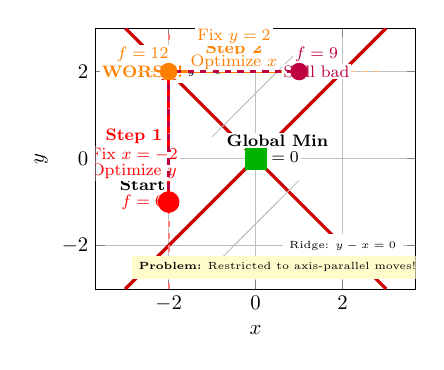
\begin{tikzpicture}[scale=0.75]
\begin{axis}[
    width=7cm, height=6cm,
    xlabel={$x$}, ylabel={$y$},
    xmin=-3, xmax=3, ymin=-3, ymax=3,
    axis equal,
    grid=major
]
% Enhanced ridge lines with labels
\draw[ultra thick, red!80!black] (-3,-3) -- (3,3);
\draw[ultra thick, red!80!black] (-3,3) -- (3,-3);
\node[fill=white] at (axis cs:-2,2) {\tiny Ridge: $x+y=0$};
\node[fill=white] at (axis cs:2,-2) {\tiny Ridge: $y-x=0$};

% Simplified contour lines to avoid parsing issues
\draw[gray!50, thin] (0.5,2) -- (-1,0.5);
\draw[gray!50, thin] (1,2.5) -- (-0.5,1);
\draw[gray!50, thin] (-0.5,-2) -- (1,-0.5);
\draw[gray!50, thin] (-1,-2.5) -- (0.5,-1);

% Starting point with clear annotation
\addplot[only marks, mark=*, mark size=5pt, color=red] coordinates {(-2, -1)};
\node[fill=white, inner sep=1pt] at (axis cs:-2.6,-0.6) {\footnotesize \textbf{Start}};
\node[fill=white, inner sep=1pt] at (axis cs:-2.6,-1.0) {\footnotesize \color{red} $f=6$};

% Step 1: Fix x=-2, optimize y - show the 1D optimization problem
\addplot[ultra thick, red, ->] coordinates {(-2,-1) (-2,2)};
\node[fill=white, inner sep=1pt] at (axis cs:-2.8,0.5) {\footnotesize \color{red} \textbf{Step 1}};
\node[fill=white, inner sep=1pt] at (axis cs:-2.8,0.1) {\footnotesize \color{red} Fix $x=-2$};
\node[fill=white, inner sep=1pt] at (axis cs:-2.8,-0.3) {\footnotesize \color{red} Optimize $y$};

% Show the vertical line for 1D optimization in Step 1
\draw[dashed, red!50, thick] (-2,-3) -- (-2,3);

% Point after step 1
\addplot[only marks, mark=*, mark size=4pt, color=orange] coordinates {(-2, 2)};
\node[fill=white, inner sep=1pt] at (axis cs:-2.6,2.4) {\footnotesize \color{orange} $f=12$};
\node[fill=white, inner sep=1pt] at (axis cs:-2.6,2.0) {\footnotesize \color{orange} \textbf{WORSE!}};

% Step 2: Fix y=2, optimize x - show the 1D optimization problem
\addplot[ultra thick, orange, ->] coordinates {(-2,2) (1,2)};
\node[fill=white, inner sep=1pt] at (axis cs:-0.5,2.5) {\footnotesize \color{orange} \textbf{Step 2}};
\node[fill=white, inner sep=1pt] at (axis cs:-0.5,2.8) {\footnotesize \color{orange} Fix $y=2$};
\node[fill=white, inner sep=1pt] at (axis cs:-0.5,2.2) {\footnotesize \color{orange} Optimize $x$};

% Show the horizontal line for 1D optimization in Step 2
\draw[dashed, orange!50, thick] (-3,2) -- (3,2);

% Point after step 2
\addplot[only marks, mark=*, mark size=4pt, color=purple] coordinates {(1, 2)};
\node[fill=white, inner sep=1pt] at (axis cs:1.4,2.4) {\footnotesize \color{purple} $f=9$};
\node[fill=white, inner sep=1pt] at (axis cs:1.4,2.0) {\footnotesize \color{purple} Still bad};

% Global minimum with emphasis
\addplot[only marks, mark=square*, mark size=5pt, color=green!70!black] coordinates {(0, 0)};
\node[fill=white, inner sep=1pt] at (axis cs:0.5,0.4) {\footnotesize \textbf{Global Min}};
\node[fill=white, inner sep=1pt] at (axis cs:0.5,0.0) {\footnotesize \textbf{$f=0$}};

% Enhanced coordinate descent path with emphasis on restriction
\draw[ultra thick, purple, dashed] (-2,-1) -- (-2,2) -- (1,2);

% Add annotations showing the constraint
\node[fill=yellow!20] at (axis cs:0.5,-2.5) {\tiny \textbf{Problem:} Restricted to axis-parallel moves!};
\end{axis}
\end{tikzpicture}
\end{figure}
\end{column}

\begin{column}{0.4\textwidth}
\begin{codebox}{Function Values}
{\small
\begin{itemize}
\item \textcolor{red}{Start $(-2,-1)$: $f=6$}
\item \textcolor{orange}{After Step 1 $(-2,2)$: $f=12$} \textcolor{orange}{$\uparrow$ WORSE}
\item \textcolor{purple}{After Step 2 $(1,2)$: $f=9$} \textcolor{purple}{Still bad}
\item \textcolor{green!70!black}{Global Min $(0,0)$: $f=0$} \textcolor{green!70!black}{$\checkmark$ Optimal}
\end{itemize}
}
\end{codebox}

\begin{alertbox}{Root Cause}
{\footnotesize
\textbf{1D Optimization Problem:}
\begin{itemize}
\item Fix $x=-2$: optimal $y$ moves away from global min
\item Fix $y=2$: optimal $x$ also suboptimal
\item Need diagonal movement!
\end{itemize}
}
\end{alertbox}
\end{column}
\end{columns}
\end{frame}

\begin{frame}{Gradient Descent vs Coordinate Descent}
\begin{columns}
\begin{column}{0.5\textwidth}
\begin{keypointsbox}{Gradient Descent}
{\footnotesize \textbf{Strategy:} Move in direction of steepest descent - can move diagonally}
\end{keypointsbox}

\begin{figure}
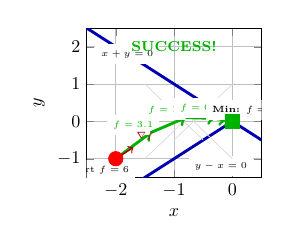
\begin{tikzpicture}[scale=0.65]
\begin{axis}[
    width=5cm, height=4.5cm,
    xlabel={$x$}, ylabel={$y$},
    xmin=-2.5, xmax=0.5, ymin=-1.5, ymax=2.5,
    grid=major
]
% Enhanced ridge lines
\draw[ultra thick, blue!70!black] (-2.5,-2.5) -- (0.5,0.5);
\draw[ultra thick, blue!70!black] (-2.5,2.5) -- (0.5,-0.5);
\node[fill=white] at (axis cs:-1.8,1.8) {\tiny $x+y=0$};
\node[fill=white] at (axis cs:-0.2,-1.2) {\tiny $y-x=0$};

% Simplified contour indication
\draw[gray!30, thin] (-1.5,-1) -- (-0.5,0.5);
\draw[gray!30, thin] (-1,-0.5) -- (0,1);
\draw[gray!30, thin] (-1.5,1) -- (-0.5,-0.5);
\draw[gray!30, thin] (-1,0.5) -- (0,-1);

% Starting point
\addplot[only marks, mark=*, mark size=4pt, color=red] coordinates {(-2, -1)};
\node[fill=white] at (axis cs:-2.3,-1.3) {\tiny Start $f=6$};

% Gradient descent path with step annotations
\addplot[ultra thick, green!70!black, ->] coordinates {(-2,-1) (-1.4,-0.3)};
\node[fill=white] at (axis cs:-1.7,-0.1) {\tiny \color{green!70!black} $f=3.1$};
\addplot[ultra thick, green!70!black, ->] coordinates {(-1.4,-0.3) (-0.8,0.1)};
\node[fill=white] at (axis cs:-1.1,0.3) {\tiny \color{green!70!black} $f=1.5$};
\addplot[ultra thick, green!70!black, ->] coordinates {(-0.8,0.1) (-0.3,0.08)};
\node[fill=white] at (axis cs:-0.55,0.35) {\tiny \color{green!70!black} $f=0.7$};
\addplot[ultra thick, green!70!black, ->] coordinates {(-0.3,0.08) (-0.1,0.03)};
\addplot[ultra thick, green!70!black, ->] coordinates {(-0.1,0.03) (0,0)};

% Global minimum
\addplot[only marks, mark=square*, mark size=4pt, color=green!70!black] coordinates {(0, 0)};
\node[fill=white] at (axis cs:0.2,0.3) {\tiny \textbf{Min: $f=0$}};
\node at (axis cs:-1,2) {\footnotesize \color{green!70!black} \textbf{SUCCESS!}};

% Show gradient arrows at starting point
\draw[->, thick, red!70!black] (axis cs:-2,-1) -- (axis cs:-1.7,-0.7);
\node at (axis cs:-1.5,-0.4) {\tiny \color{red!70!black} $\nabla f$};
\end{axis}
\end{tikzpicture}
\end{figure}
\end{column}

\begin{column}{0.5\textwidth}
\begin{alertbox}{Coordinate Descent}
{\footnotesize \textbf{Constraint:} Only axis-parallel moves - gets trapped!}
\end{alertbox}

\begin{figure}
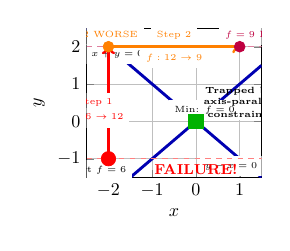
\begin{tikzpicture}[scale=0.65]
\begin{axis}[
    width=5cm, height=4.5cm,
    xlabel={$x$}, ylabel={$y$},
    xmin=-2.5, xmax=1.5, ymin=-1.5, ymax=2.5,
    grid=major
]
% Enhanced ridge lines
\draw[ultra thick, blue!70!black] (-2.5,-2.5) -- (1.5,1.5);
\draw[ultra thick, blue!70!black] (-2.5,2.5) -- (1.5,-1.5);
\node[fill=white] at (axis cs:-1.8,1.8) {\tiny $x+y=0$};
\node[fill=white] at (axis cs:0.8,-1.2) {\tiny $y-x=0$};

% Show the constraint lines for 1D optimization
\draw[dashed, red!50, thick] (-2.5,-1) -- (1.5,-1);
\draw[dashed, orange!50, thick] (-2,-1.5) -- (-2,2.5);
\draw[dashed, purple!50, thick] (-2.5,2) -- (1.5,2);

% Starting point
\addplot[only marks, mark=*, mark size=4pt, color=red] coordinates {(-2, -1)};
\node[fill=white] at (axis cs:-2.3,-1.3) {\tiny Start $f=6$};

% Coordinate descent moves with function values
\addplot[ultra thick, red, ->] coordinates {(-2,-1) (-2,2)};
\node[fill=white] at (axis cs:-2.3,0.5) {\tiny \color{red} Step 1};
\node[fill=white] at (axis cs:-2.3,0.1) {\tiny \color{red} $f: 6 \to 12$};

\addplot[only marks, mark=*, mark size=3pt, color=orange] coordinates {(-2, 2)};
\node[fill=white] at (axis cs:-2.3,2.3) {\tiny \color{orange} $f=12$ WORSE};

\addplot[ultra thick, orange, ->] coordinates {(-2,2) (1,2)};
\node[fill=white] at (axis cs:-0.5,2.3) {\tiny \color{orange} Step 2};
\node[fill=white] at (axis cs:-0.5,1.7) {\tiny \color{orange} $f: 12 \to 9$};

\addplot[only marks, mark=*, mark size=3pt, color=purple] coordinates {(1, 2)};
\node[fill=white] at (axis cs:1.3,2.3) {\tiny \color{purple} $f=9$ Bad};

% Global minimum
\addplot[only marks, mark=square*, mark size=4pt, color=green!70!black] coordinates {(0, 0)};
\node[fill=white] at (axis cs:0.2,0.3) {\tiny Min: $f=0$};
\node at (axis cs:0,-1.3) {\footnotesize \color{red} \textbf{FAILURE!}};

% Show axis-parallel constraint
\node at (axis cs:1,0.8) {\tiny \textbf{Trapped by}};
\node at (axis cs:1,0.5) {\tiny \textbf{axis-parallel}};
\node at (axis cs:1,0.2) {\tiny \textbf{constraint!}};
\end{axis}
\end{tikzpicture}
\end{figure}
\end{column}
\end{columns}
\end{frame}

\begin{frame}{Why Coordinate Descent Fails Here}
\begin{alertbox}{Problem}
Function $f(x, y) = |x + y| + 3|y - x|$ is non-separable
\end{alertbox}

\begin{codebox}{Analysis}
{\small
\begin{itemize}
\item Start at $(-2, -1)$: $f(-2, -1) = |-3| + 3|-1| = 6$
\item Fix $x = -2$, optimize $y$: optimal $y = 2$
\item New point $(-2, 2)$: $f(-2, 2) = 12$ (worse!)
\end{itemize}
}
\end{codebox}
\end{frame}

\begin{frame}{When Coordinate Descent Fails}
\begin{theorembox}{Failure Conditions}
{\small
\begin{itemize}
\item Non-separable functions
\item Strong coupling between variables
\item Need simultaneous movement in multiple directions
\end{itemize}
}
\end{theorembox}

\begin{keypointsbox}{Fortunately}
Lasso objective IS separable, so coordinate descent works well!
\end{keypointsbox}
\end{frame}

\begin{frame}{Coordinate Descent for Unregularised Regression}

\begin{itemize}[<+->]
	
	
	
	
	
	\item Express error as a difference of $y_{i}$ and $\hat{y_{i}}$
	\begin{equation}
	\hat{y_i} = \sum_{j=0}^{d} \theta_{j}x^{j}_{i} = \theta_{0}x_{i}^{0} + \theta_{1}x_{i}^{1} +\theta_{2}x_{i}^{2} + \ldots + \theta_{d}x_{i}^{d}
	\end{equation}
	\begin{equation}
	\epsilon_{i} = y_{i} - \hat{y_{i}} = y_{i} - \theta_{0}x_{i}^{0} - \theta_{1}x_{i}^{1} - \ldots - \theta_{d}x_{i}^{d} = y_{i} - \sum_{j=0}^{d} \theta_{j}x_{i}^{j}
	\end{equation}
	
	
	
\end{itemize}


\end{frame}



\begin{frame}{Coordinate Descent for Unregularised regression}

\[
\sum_{i=1}^{n}  \epsilon^{2}=\RSS =\sum_{i=1}^{n}\left(y_{i}-\left(\theta_{0}x_{i}^{0}+\ldots + \theta_{j} x_{i}^{j}+\theta_{d} x_{i}^{d}\right)\right)^{2}
\]
\end{frame}

\begin{frame}{Coordinate Descent for Unregularised regression}

\[
\sum_{i=1}^{n}  \epsilon^{2}=\RSS =\sum_{i=1}^{n}\left(y_{i}-\left(\theta_{0}x_{i}^{0}+\ldots + \theta_{j} x_{i}^{j}+\theta_{d} x_{i}^{d}\right)\right)^{2}
\]
\[
\frac{\partial \RSS\left(\theta_{j}\right)}{\partial \theta_{j}}= 2 \sum_{i=1}^{n}\left(y_{i}-\left(\theta_{0}x_{i}^{0}+\ldots + \theta_{j} x_{i}^{j}+\ldots \right)\right)\left(-x_{i}^{j}\right)
\]
\end{frame}

\begin{frame}{Coordinate Descent for Unregularised regression}

\[
\sum_{i=1}^{n}  \epsilon^{2}=\RSS =\sum_{i=1}^{n}\left(y_{i}-\left(\theta_{0}x_{i}^{0}+\ldots + \theta_{j} x_{i}^{j}+\theta_{d} x_{i}^{d}\right)\right)^{2}
\]
\[
\frac{\partial \RSS\left(\theta_{j}\right)}{\partial \theta_{j}}= 2 \sum_{i=1}^{n}\left(y_{i}-\left(\theta_{0}x_{i}^{0}+\ldots + \theta_{j} x_{i}^{j}+\ldots \right)\right)\left(-x_{i}^{j}\right)
\]
\[
=2\sum_{i=1}^{n}\left(y_{i}-\left(\theta_{0} x_{i}^{0}+\ldots + \theta_{d} x_{i}^{d}\right)\right)\left(-x_{i}^{j}\right)+2 \sum_{i=1}^{n} \theta_{j}(x_{i}^j)^2
\]
\pause where: $$\hat{y_{i}}^{(-j)} = \theta_{0} x_{i}^{0}+\ldots + \theta_{d} x_{i}^{d}$$ is $\hat{y}_{i}$ without $\theta_{j}$
\end{frame}

\begin{frame}{Coordinate Descent for Unregularised regression}

\[
\text{Set } \frac{\partial \RSS\left(\theta_{j}\right)}{\partial \theta_{j}}= 0
\]
\[
\theta_{j}=\sum_{i=1}^{n} \frac{\left(y_{i}-\left(\theta_{0} x_{i}^{0}+\ldots + \theta_{d} x_{i}^{d}\right)\right)\left(x_{i}^{j}\right)}{\left(x_{i}^{j}\right)^{2}}= \frac{\rho_{j}}{z_{j}}
\]
\[
\rho_{j} =\sum_{i=1}^{n} x_{i}^{j}\left(y_{i}-{\hat{y}_{i}^{(-j)}}\right) \quad \text{and} \quad z_{j}=\sum_{i=1}^{n}\left(x_{i}^{j}\right)^{2}
\]
$z_{j}$ is the squared of $\ell_2$ norm of the $j^{th}$ feature
\end{frame}

%{
%\setbeamercolor{background canvas}{bg=}
%\includepdf[page=-]{coordinate-rho.pdf}
%}




\section{Mathematical Derivation}

\begin{frame}{Lasso Coordinate Descent: Setup}
\begin{codebox}{Lasso Objective}
$$\text{Minimize } \underbrace{\sum_{i=1}^{n} (y_i - \hat{y}_i)^{2} + \lambda \sum_{j=0}^{d} |\theta_{j}|}_{\text{Lasso Objective}}$$
\end{codebox}
\pause

\begin{keypointsbox}{Key Definitions}
\begin{itemize}
\item $\rho_j = \sum_{i=1}^{n} x_{ij}(y_i - \hat{y}_i^{(-j)})$ (partial residual correlation)
\item $z_j = \sum_{i=1}^{n} x_{ij}^2$ (feature norm squared)
\item $\hat{y}_i^{(-j)} = $ prediction without $j$-th feature
\end{itemize}
\end{keypointsbox}
\end{frame}

\begin{frame}{Coordinate Descent: Subgradient Analysis}
\begin{codebox}{Subgradient of Lasso Objective w.r.t. $\theta_j$}
$$\frac{\partial}{\partial \theta_{j}}(\text{Lasso Objective}) = -2\rho_{j} + 2\theta_{j}z_{j} + \lambda \frac{\partial}{\partial \theta_{j}}|\theta_{j}|$$
\end{codebox}
\pause

\begin{theorembox}{Subgradient of $|\theta_j|$}
$$\frac{\partial}{\partial \theta_{j}}|\theta_{j}| = \begin{cases}
+1 & \text{if } \theta_{j} > 0 \\
[-1,+1] & \text{if } \theta_{j} = 0 \\
-1 & \text{if } \theta_{j} < 0
\end{cases}$$
\end{theorembox}
\end{frame}

\begin{frame}{Case Analysis: $\theta_j > 0$}
\begin{codebox}{Case 1: $\theta_j > 0$}
Subgradient is $+1$, so optimality condition:
$$-2\rho_j + 2\theta_j z_j + \lambda = 0$$
\end{codebox}
\pause

\begin{theorembox}{Solution}
$$\theta_j = \frac{\rho_j - \lambda/2}{z_j}$$
This is valid when $\rho_j > \lambda/2$ (ensures $\theta_j > 0$)
\end{theorembox}
\pause

\begin{alertbox}{Soft Thresholding}
Notice the $-\lambda/2$ term: this "shrinks" the coefficient!
\end{alertbox}
\end{frame}

\begin{frame}{Case Analysis: $\theta_j < 0$}
\begin{codebox}{Case 2: $\theta_j < 0$}
Subgradient is $-1$, so optimality condition:
$$-2\rho_j + 2\theta_j z_j - \lambda = 0$$
\end{codebox}
\pause

\begin{theorembox}{Solution}
$$\theta_j = \frac{\rho_j + \lambda/2}{z_j}$$
This is valid when $\rho_j < -\lambda/2$ (ensures $\theta_j < 0$)
\end{theorembox}
\pause

\begin{alertbox}{Symmetric Shrinkage}
Same shrinkage effect, but in the opposite direction!
\end{alertbox}
\end{frame}

\begin{frame}{Case Analysis: $\theta_j = 0$}
\begin{codebox}{Case 3: $\theta_j = 0$}
Subgradient $\in [-1,+1]$, so optimality requires:
$$0 \in [-2\rho_j - \lambda, -2\rho_j + \lambda]$$
\end{codebox}
\pause

\begin{theorembox}{Zero Condition}
This happens when:
$$-2\rho_j - \lambda \leq 0 \text{ and } -2\rho_j + \lambda \geq 0$$
$$\Rightarrow -\frac{\lambda}{2} \leq \rho_j \leq \frac{\lambda}{2}$$
\end{theorembox}
\pause

\begin{alertbox}{Sparsity Mechanism}
If correlation $|\rho_j|$ is small ($ \leq \lambda/2$), set $\theta_j = 0$!
\end{alertbox}
\end{frame}
\begin{frame}{Soft-Thresholding Operator}
\begin{definitionbox}{Complete Lasso Update Rule}
{\small
$$\theta_{j} = \begin{cases}
\frac{\rho_{j} + \lambda/2}{z_{j}} & \text{if } \rho_{j} < -\lambda/2 \\
0 & \text{if } |\rho_{j}| \leq \lambda/2 \\
\frac{\rho_{j} - \lambda/2}{z_{j}} & \text{if } \rho_{j} > \lambda/2
\end{cases}$$
}
\end{definitionbox}
\end{frame}

\begin{frame}{Soft-Thresholding Properties}
\begin{keypointsbox}{Key Properties}
{\small
\begin{itemize}
\item \textbf{Shrinkage}: Coefficients pulled toward zero
\item \textbf{Selection}: Small coefficients $\rightarrow$ exactly zero
\item \textbf{Soft-thresholding}: Smooth shrinkage + selection
\end{itemize}
}
\end{keypointsbox}

\begin{examplebox}{Intuition}
Weak correlation $|\rho_j| \leq \lambda/2$ $\Rightarrow$ eliminate feature!
\end{examplebox}
\end{frame}

\section{Lasso vs Ridge Comparison}

\begin{frame}{Lasso vs Ridge: Key Differences}
\begin{table}[h]
\centering
\begin{tabular}{|l|c|c|}
\hline
\textbf{Property} & \textbf{Ridge (L2)} & \textbf{Lasso (L1)} \\
\hline
Penalty & $\sum \theta_j^2$ & $\sum |\theta_j|$ \\
\hline
Sparsity & Never exactly zero & Can be exactly zero \\
\hline
Feature Selection & No & Yes \\
\hline
Differentiable & Yes & No (at $\theta_j = 0$) \\
\hline
Solution Method & Closed form & Coordinate descent \\
\hline
Constraint Shape & Circle & Diamond \\
\hline
Best for & Multicollinearity & Feature selection \\
\hline
\end{tabular}
\end{table}
\end{frame}

\begin{frame}{When to Use Lasso vs Ridge}
\begin{keypointsbox}{Use Lasso When:}
\begin{itemize}
\item High-dimensional data ($p >> n$)
\item Need interpretable model
\item Expect only few features are truly relevant
\item Want automatic feature selection
\end{itemize}
\end{keypointsbox}
\pause

\begin{keypointsbox}{Use Ridge When:}
\begin{itemize}
\item All features might be somewhat relevant
\item Multicollinearity is the main problem
\item Want to keep all features with reduced impact
\item Need stable solution with correlated features
\end{itemize}
\end{keypointsbox}
\end{frame}

\section{Summary and Applications}

\begin{frame}{Lasso Regression: Summary}
\begin{definitionbox}{Lasso in a Nutshell}
Lasso = Linear regression + L1 penalty for automatic feature selection
\end{definitionbox}

\begin{keypointsbox}{Key Advantages}
{\small
\begin{itemize}
\item ✅ Regression + feature selection simultaneously
\item ✅ Sparse, interpretable models
\item ✅ Handles high-dimensional data well
\end{itemize}
}
\end{keypointsbox}
\end{frame}

\begin{frame}{Lasso: Limitations and Applications}
\begin{keypointsbox}{Limitations}
{\small
\begin{itemize}
\item ❌ Arbitrary selection among correlated features
\item ❌ May underperform when all features are relevant
\end{itemize}
}
\end{keypointsbox}

\begin{examplebox}{Applications}
Genomics, text mining, signal processing, finance, marketing analytics
\end{examplebox}
\end{frame}

\end{document}
